\section{Browser Security Warnings and HTTPS Errors}
%����Ҫ��дһ���ܽ���ܵĻ�
\subsection{Browser Security Warnings}
Browser uses security warnings to protect users by alerting them to network attacks. 
    According to different levels of risk, 
    Browser presents different connection security states in order to maximize security and minimize side effects of user experience. We describe security warnings of major browsers.

\subsubsection{Risk Level A: Low-risk warnings}
In this scenario, a passive security indicator indicates minor HTTPS errors by removing lock icon, changing lock icon��s color, providing textual information, or by other means without interrupting the user��s browsing.
\begin{figure}[htbp]
\centerline{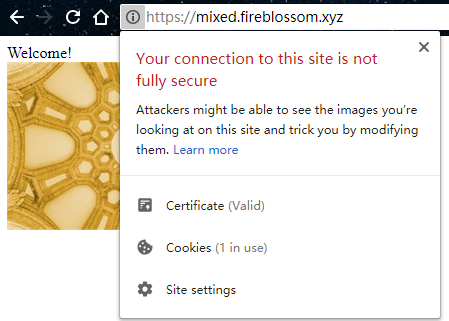
\includegraphics[height=3cm,width=7cm]{Figure/fig1.png}}%�ǵû���chrome�Ľ�ͼ
\caption{low-risk warning in chrome.}
\label{fig}
\end{figure}
this is probably because webmaster has configured his website correctly, including purchasing a valid certificate, but the website still contains images or scripts over plain HTTP. Although the browser was able to establish a valid HTTPS connection, there are still minor problems.

\subsubsection{Risk Level B: Medium-risk warnings that can be bypassed}
Bypassable HTTPS security warnings are the most common type of browser warning. Browsers use bypassable HTTPS security warning to treat the vast majority of HTTPS errors.
\begin{figure}[htbp]
\centerline{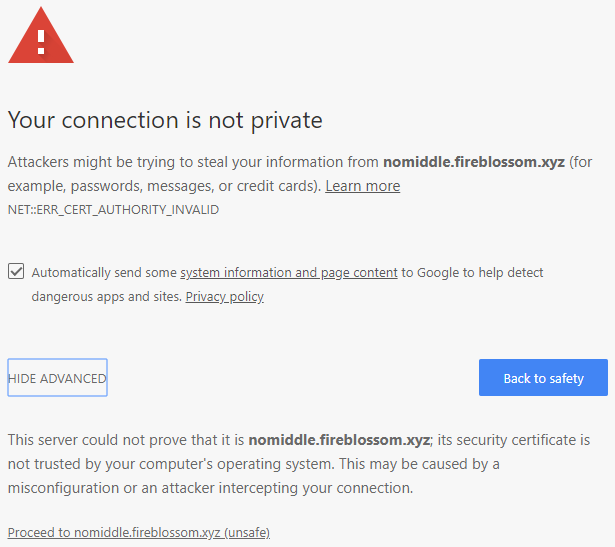
\includegraphics[height=3cm,width=7cm]{Figure/fig2.png}}
\caption{medium-risk warning in chrome.}
\label{fig}
\end{figure}
In this scenario, if there is an HTTPS error, the browser will stop the page load and display an HTTPS security warning. Typically, users are able to click through the warning by clicking on a button, but this may be disabled if the website servers the HTTP Strict Transport Security (HSTS) or HTTP Public Key Pinning (HPKP) header. Although the HTTP(s) traffic we captured through Fiddler[ https://www.telerik.com/fiddler] shows the web page is not transmitted in plain text, clicking through the warning may allow an actual man-in-the-middle attack to proceed.

\subsubsection{Risk Level C: High-risk warnings that cannot be bypassed}
As a worst case scenario, the browser will prevent uses from continuing to browse the website by showing a security warning that the users cannot bypass.
\begin{figure}[htbp]
\centerline{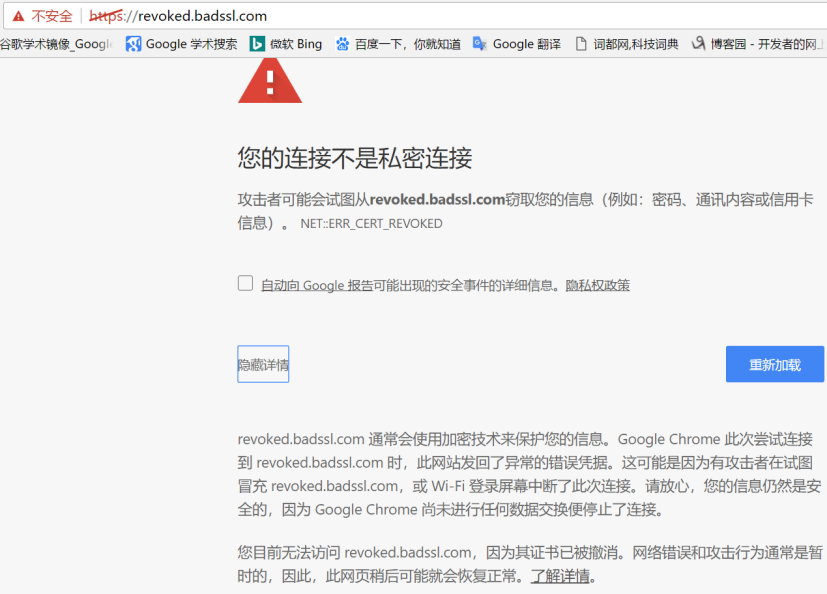
\includegraphics[height=3cm,width=7cm]{Figure/fig3.png}}%�ǵû����Լ�fireblossom.xyz��ַ�Ľ�ͼ
\caption{high-risk warning in chrome.}
\label{fig}
\end{figure}
this is probably because the website is supposed to establish a valid HTTPS connection, but the certificate chain fails to validate (e.g., a HTTPS certificate error occurs in a website that has deployed HSTS policy).

\subsubsection{Cannot establish HTTPS connection}
The browser may fail to establish a HTTPS connection to the server for unsupported TLS version, cipher mismatch, or other reasons. In this scenario, the browser cannot obtain certificates from the web server, let alone certificate validation, so the TLS handshake error is not discussed in this paper.
\begin{figure}[htbp]
\centerline{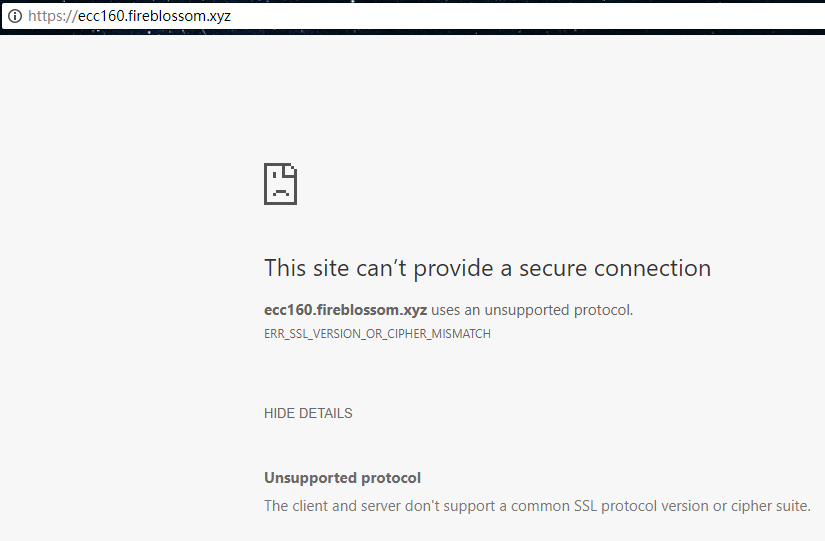
\includegraphics[height=3cm,width=7cm]{Figure/fig4.png}}%��ͼ��Ҫ�ٵ�����������
\caption{Cannot establish HTTPS connection in chrome.}
\label{fig}
\end{figure}
